

%% La classe stageM2R s'appuie sur la classe memoir, plus d'information sur le paquet: http://www.ctan.org/pkg/memoir
%% option possible de la classe stageM2R
% utf8  -> encodage du texte UTF8 (défaut: Latin1)
% final -> mode rapport de stage final (défaut: mode étude bibliographique)
% private -> indique une soutenance privée (défaut: soutenance publique)
\documentclass[utf8]{stageM2R} %-> etude bibliographique
%\documentclass[utf8,final]{stageM2R} %-> rapport final

\usepackage{amsmath}
\usepackage{graphicx}
\usepackage[colorinlistoftodos]{todonotes}
\usepackage{todonotes}
\usepackage[babel=true]{csquotes} % csquotes va utiliser la langue définie dans babel
\usepackage{amsthm}
 \usepackage{multicol}
\newtheorem{mydef}{Définition}
\theoremstyle{remark}
\renewcommand{\emph}{\textbf}
\newenvironment{exemple}{%
\upshape Exemple :% Environnement quote
   % ... en italique
    \small     % ... en plus petit
}{%
}

%%%%%%%%%%%%%%%%%%%%%%%%%%%%
%%% Déclaration du stage %%%
%%%%%%%%%%%%%%%%%%%%%%%%%%%%

%% auteur
\author{Cédric \bsc{Maigrot}}
%% encadrants
\supervisors{Sandra \bsc{Bringay}\\Jérôme \bsc{Azé}}
%% lieu du stage (Optionnel)
\location{LIRMM UM5506 - CNRS, Université de Montpellier}
%% titre du stage
\title{Prévention du risque de suicide via les réseaux sociaux\\Détection de points de rupture dans le comportement des personnes à risques} 
%% parcours du master
\track{DECOL}  
%% date de soutenance (Optionnel)
\date{\today} 
%% version du rapport (Optionnel)
\version{5}
%% Résumé en francais
\abstractfr{
Le suicide devient d'année en année une problématique plus préoccupante. Les organismes de santé (l'OMS et l'ONS) se sont engagés à réduire le nombre de suicide de 10\% dans l'ensemble des pays d'ici 2020. Même si le suicide est un geste impulsif, il existe souvent des comportements et des paroles qui peuvent révéler un mal être et être des signes précurseurs de prédispositions au suicide. L'objectif de ce stage est de mettre en place un système pour détecter semi-automatiquement ces comportements et ces paroles au travers des réseaux sociaux.

Des travaux précédents \cite{Abboute2014} ont proposé le classement de messages issus de Twitter suivant des thèmes liés au suicide : tristesse, blessures psychologiques, état mental,  dépression,  peur,  solitude,  description de la tentative de suicide,  anorexie, réactions aux insultes et cyber-harcèlement. Dans ce stage, l'étude se focalise plus précisément sur la réaction des jeunes au sujet du cyber-harcèlement. Nous étudierons notament des messages anonymisés de jeunes qui contactent  l'Organisme Arrêt Demandé International (OADI), spécialisé dans l'aide aux personnes victimes de harcèlement. La 1ère partie de cette bibliographie portera sur les méthodes d'analyse de sentiments.

Outre les problèmes classiques liés à l'analyse des textes mal rédigés issus des réseaux sociaux, un des principaux challenge de ce stage est de mettre en place un système de gestion des flux de données. De nouveaux messages pouvent apparaître à tout moment et doivent être pris en compte dans l'analyse. Cela implique la mise en place de techniques spécifiques  telles que le \textit{concept drift} sur lequel portera la 2e partie de cet état de l'art et qui permettront de capter l'apparition d'un nouveau sentiment comme la peur.

\emph{Mots clés : } Analyse de sentiments, Flux de données, Concept drift
}
%% Résumé en anglais
\abstracteng{
  This master thesis.
}


\begin{document}   
%\selectlanguage{english} %% --> turn the document into english mode (Default is french)
\selectlanguage{french} 
\frontmatter  %% -> pas de numérotation numérique
\maketitle    %% -> création de la page de garde et des résumés
\cleardoublepage   
\tableofcontents %% -> table des matières
\mainmatter  %% -> numérotation numérique	


%%%%%%%%%%%%%%%%%%%%%%%%%%%%%%
%%%%    DEBUT DU RAPPORT  %%%%
%%%%%%%%%%%%%%%%%%%%%%%%%%%%%%

%%%%%%%%%%%%%%%%%%%%%%%%%%%%%%
%%%%    chapitre CONTEXTE  %%%%
%%%%%%%%%%%%%%%%%%%%%%%%%%%%%%
\chapter{Contexte}
\enquote{Le suicide est évitable. Pourtant, toutes les 40 secondes, une personne se suicide quelque part dans le monde et bien plus tente de mettre fin à ses jours. Toutes les régions et toutes les  tranches d’âge sont touchées, notamment  les jeunes de 15 à 29 ans, pour qui le suicide est la deuxième cause de mortalité à l’échelle mondiale}\footnote{Prévention du suicide, L'état d'urgence mondial. OMS 2014. ISBN: 978 92 4 256477 8}. Le constat au niveau national, avec le premier rapport annuel de l'Observatoire National du Suicide (ONS) en décembre 2014, est identique\footnote{Marisol Touraine reçoit le premier rapport annuel de l'Observatoire national du suicide - Ministère des Affaires sociales, de la Santé et des Droits des femmes - http://www.sante.gouv.fr/marisol-touraine-recoit-le-premier-rapport-annuel-de-l-observatoire-national-du-suicide.html}. Des mesures de prévention sont mises en place par les organismes de santé car le suicide devient un problème majeur.

Parmi les principales causes de suicide, on trouve le harcèlement. Lors d'un harcèlement "ordinaire", la victime est harcelée sur un lieu précis (école, travail, bus, \dots). Alors que dans le cas d'un \emph{cyber-harcèlement}, les messages vont continuer sur  Facebook, Twitter ou tout autre réseau social que l'on serait amené à fréquenter en étant en dehors du lieu de harcèlement. Il n'existe alors plus de répit pour la victime qui se retrouve dans un contexte d'oppression menant parfois au suicide. Dans le cadre de ce stage, l'étude portera spécifiquement sur les liens entre cyber-harcèlement et idéations suicidaires.

L'Organisme Arrêt Demandé International\footnote{http://oadi.education/presentation/} (OADI), vient en aide aux personnes victimes de harcèlement. Il étudie le phénomène du harcèlement à l'école dans douze pays grâce à ses filiales associatives internationales. Leur but est de comprendre comment le phénomène du harcèlement scolaire est appréhendé dans les autres pays du monde afin d'améliorer son approche établie en France. L'OADI met à notre disposition des messages de jeunes les contactant et pouvant exprimer des idéations suicidaires. 

Le but du stage est de parvenir à prédire les points de rupture dans le comportement des personnes suite à un cyber-harcèlement. Les résultats pourront être appliqués aux futurs messages reçus par OADI, mais aussi plus généralement sur des comptes d'utilisateurs de réseaux sociaux. Pour mener à bien ce projet, il sera nécessaire de se focaliser sur trois aspects : 1) la détection des harcèlements; 2) la détection des sentiments exprimés par la personne harcelée; 3) la détection des \textit{concept drifts} sur ces sentiments (e.g. l'apparition d'un sentiment de perte d'estime de soi). Ce rapport étant  court, nous ne décrirons pas le premier aspect mais le travail bibliographique a également été réalisé. On peut citer par exemple les  méthodes de \cite{Nahar2012} ou de  \cite{Yin2009}. Les deux autres aspects seront traités dans les sections \ref{AnalyseSemantique} et \ref{ConceptDrift}.

%%%%%%%%%%%%%%%%%%%%%%%%%%%%%%
%%%%    chapitre ANALYSE SEMANTIQUE  %%%%
%%%%%%%%%%%%%%%%%%%%%%%%%%%%%%

\chapter{Analyse de sentiments}\label{AnalyseSemantique}

Dans cette section, nous nous intéressons aux méthodes d'analyse de sentiments pouvant être appliquées pour capturer l'humeur des personnes harcelées.
On distingue les méthodes portant sur la polarité (e.g. positive, négative) et sur les émotions (joie, colère,  \dots) qui nous intéresserons plus particulièrement.
Nous décrivons dans la suite trois catégories de méthodes : 1) \emph{Analyse fréquentielle}, en rapport à la fréquence d'apparition d'un mot; 2) \emph{Génération de règles}, en produisant des règles qui associent un ensemble de mots à un sentiment; 3) \emph{Apprentissage}, pour apprendre  des modèles permettant de prédire des classes de sentiments pour de nouvelles instances. Nous  nous focalisons sur celles liées soit à la détection des maladies mentales, soit aux flux de textes.

\section{Détection par analyse fréquentielle}
Une des techniques les plus utilisées est la pondération $TF-IDF$ \cite{Salton1988}. Pour trouver le(s) mot(s) significatif(s) dans un texte, on utilise d'une part l'occurrence du mot dans un texte (Term Frequency - $TF$) et d'autre part le nombre de documents  contenant ce mot  (Inverse Documents Frequency - $IDF$). Un mot très fréquent dans un texte, mais peu présent dans un ensemble de textes, ne sera pas significatif. À l'inverse, un mot très fréquent dans un texte mais présent que dans ce texte sera utilisé pour le décrire.
Lors d'une analyse avec des données sous forme de flux comme dans notre étude, l'utilisation de $TF-IDF$ est difficile car le calcul de $IDF$ nécessite de connaître le nombre de textes. Pour les flux de documents, \cite{Reed2006} propose de remplacer $IDF$ par $ICF$  (Inverse Corpus Frequency - $ICF$), le calcul de $ICF$ est le même que $IDF$ mais en se basant sur le corpus statique et non sur l'intégralité des textes du flux. Cela a pour effet d'approximer la valeur obtenue par $IDF$ tout en gardant un faible temps de calcul.
\cite{Pennebaker2001} propose une autre approche fréquentielle grâce à $Linguistic~Inquiry~and~Word~Count~(LIWC)$, un méthode qui calcule le degré selon lequel les personnes utilisent différentes catégories de mots dans un ensemble de textes. Il permet aussi de classer les textes selon une émotion positive ou négative. Cette méthode a été utilisée dans \cite{Gunn2012} pour analyser les messages laissés sur Twitter avant un suicide.
Pour finir, les émoticones, ou \texttt{smileys}, sont très utilisés dans les réseaux sociaux pour exprimer les émotions liées à la phrase ou au message écrit. Ils peuvent être utilisés comme  un mot de la phrase. \cite{Hogenboom2013} propose un lexique d'émoticones, ce qui a pour résultat d'augmenter la précision des méthodes de classification. \cite{Read2005} montre qu'avec la prise en compte des émoticones, les règles construites par le système d'apprentissage se simplifient.

\section{Détection par génération de règles}
\cite{Silva2011a} présente une méthodologie pour rattacher un sentiment à un texte dans le cas d'une analyse en streaming. À partir de quelques exemples annotés, des règles d'associations sont générées pour créer un premier modèle. Ces règles sont stockées sous la forme de couple clé/valeur où la clé est la règle et la valeur est le triplet $\sigma(X)$,$\sigma(X\cup s_i)$ et $\theta(X\rightarrow s_i)$ qui représentent respectivement le support de X (i.e. le nombre de règles ayant $X$ en corps de règle), le support de $X$ et $s_i$ (i.e. le nombre de règles ayant $X$ en corps de règle et $s_i$ en tête de règle) et la confiance  de $X\rightarrow s_i$ donnée par $\theta(X\rightarrow s_i) = \frac{\sigma(X\cup s_i)}{\sigma(X)}$. Grâce à ces valeurs, il est possible d'une part de vérifier rapidement si un nouveau texte correspond à un sentiment connu ou non, et d'autre part, de maintenir à jour le modèle en incrémentant les valeurs correspondantes et sans les recalculer constamment. Lors de la classification d'un nouveau texte, il est possible d'extraire de nouvelles règles pour mettre à jour le modèle. Celles-ci sont conservées si elles obtiennent une confiance supérieure à un seuil fixé par l'utilisateur. Un seuil de confiance élevé préserve des règles de haute qualité mais qui sont trop sélectives et trop peu souvent applicables.

\section{Détection par apprentissage}
Le principe des méthodes par apprentissage (\texttt{machine learning}) consiste à déduire un modèle à partir d'un corpus de textes donné en exemple dans lequel le système  va apprendre des régularités. On distingue  trois types de méthodes : 1) L'\emph{Apprentissage supervisé}
 permet une classification des données à partir d'un corpus annoté (i.e. possédant l'information de la classe à laquelle le message appartient) qui permet de construire un modèle. Le système peut alors classer les nouveaux textes grâce à ce modèle. \cite{Abboute2014} identifie ainsi sur Twitter des messages à risques suicidaires; 2)  À l'inverse, un \emph{Apprentissage non-supervisé}  commence  avec un ensemble non annotés. Le système  identifie des structures récurrentes à partir desquelles un modèle est construit de manière à ce que les données considérées comme les plus similaires soient associées au sein d'un groupe homogène et qu'au contraire les données considérées comme différentes se retrouvent dans d'autres groupes distincts. Dans le cas d'une analyse de polarité, cette approche se montre efficace lors d'un classement en deux groupes  (i.e. un cluster pour les messages positifs et un autre les négatifs) \cite{Li2014}. Cependant, l'apprentissage non-supervisé peut aussi s'appliquer à des émotions \cite{Kim2010}.  3) Les approches d'\emph{Apprentissage semi-supervisé} se basent sur l'utilisation d'un corpus annoté et d'un second non-annoté. Le principe de l'apprentissage semi-supervisé est de modifier ou de réorganiser les hypothèses effectuées sur le modèle à partir des données d'apprentissage \cite{Ortigosa-Hernandez2012}.
%réalise un apprentissage semi-supervisé multi-dimensionnel (Plusieurs variables cibles sont utilisées).

\subsection{Synthèse}
Ces méthodes permettent d'associer un sentiment à un texte. Bien que  performantes indépendamment, les meilleurs résultats sont généralement obtenus en les utilisant  des approches hybrides comme \cite{Prabowo2009}.  Dans notre étude nous souhaiterons considérer l'évolution de ces concepts au cours du temps. Pour cela, nous nous intéresserons au \texttt{concept drift}. \textit{Comment mesurer l'évolution, l'apparition d'un concept, par exemple, l'apparition ou la disparition du concept de défaut d'estime de soi au fil des messages d'un jeune harcelé ?}

%%%%%%%%%%%%%%%%%%%%%%%%%%%%%%
%%%%    chapitre Concept drift  %%%%
%%%%%%%%%%%%%%%%%%%%%%%%%%%%%%

\chapter{Concept drift} \label{ConceptDrift}
\section{Définitions}
\label{definitions}
\subsection{Concept drift}
Dans cette partie seront énoncées les notions indispensables pour comprendre les différents aspects du \emph{concept drift}. Ces définitions sont extraites et réécrites à partir de l'article de référence \cite{Gama2014}. Pour illustrer ces définitions, elles seront accompagnées par un exemple tiré de la situation suivante :
\begin{exemple}
On étudie les pratiques sportives intéressant les utilisateurs du réseau social Twitter. Initialement, le modèle distingue les utilisateurs qui suivent deux sports, à savoir le football et la natation.
\end{exemple}


\begin{mydef}[Variable cible]
Lors d'un processus de classification, la \emph{variable cible}~$Y$ est la donnée que l'on souhaite prédire. 
\begin{exemple}
La variable cible est ici le sport que suit l'utilisateur.
\end{exemple}
\end{mydef}

\begin{mydef}[Concept]
Un \emph{concept} $y$ désigne une modalité (parmi les $c$ modalités) de la variable cible à laquelle les exemples peuvent être assignés. 
\begin{exemple}
Deux concepts sont associés à la variable cible \texttt{sport} : football et natation.
\end{exemple}
\end{mydef}


\begin{mydef}[Exemple]
Un \emph{exemple} $X$ désigne une instance. On différenciera un exemple d'apprentissage associé à un concept d'un exemple de test pour lequel le concept est à prédire.
\begin{exemple}
Un exemple d'apprentissage est un message écrit par une personne et associé au concept football et un exemple de test est un message pour lequel on n'a pas cette information.
\end{exemple}
\end{mydef}



\begin{mydef}[Feature]
Un \emph{feature} $f$ est une caractéristique d'un exemple qui est utilisée pour l'apprentissage. On parlera du feature $f_i$ pour désigner le $i_{eme}$ feature.
\begin{exemple}
Le nombre de mots dans le message.
\end{exemple}
\end{mydef}



\begin{mydef}[Distribution]
\label{defDistribution}
La \emph{distribution} représente la répartition des probabilités des exemples dans les concepts au cours du temps. Soit $X$ un exemple\footnote{Un exemple est représenté par l'ensemble des features qui le définissent} et $y$ un concept, alors $p(y|X)$ est la distribution de $y$ sachant $X$ (i.e. la probabilité que le concept $y$ soit associé à l'exemple $X$):
\[
p(y|X) = \frac{p(y)*p(X|y)}{P(X)}
\]
\end{mydef}

\begin{mydef}[Attribution d'un exemple à un concept]
L'attribution ou non d'un concept $y$ à un exemple $X$ dépend de la règle $p(y|X) \geq \delta$ où $\delta$ est un seuil fixé par l'utilisateur. Un seuil $\delta$ élevé permet de renforcer la cohérence d'un concept associé (forte corrélation entre l'exemple et le concept) mais sera plus difficile à atteindre. Cette règle a deux conséquences directes. Un exemple peut ne correspondre à aucun concept ($\forall y, p(y|X)~<~\delta$) et un exemple peut avoir plusieurs concepts associés.
\end{mydef}

\begin{mydef}[Concept drift]
Dans le cas d'un flux de données (stream), la classification peut se trouver erronée si la distribution de la variable cible est modifiée. Le \emph{concept drift} entre les instants $t_0$ et $t_1$ peut être défini comme : $\exists X : p_{t_0}(y|X) \ne p_{t_1}(y|X)$ 
où $ p_{t}(X,y)$ désigne la distribution au temps $t$ entre l'ensemble $X$ de données et la variable cible $y$.
\end{mydef}

\begin{mydef}[Prédiction]
Lors du traitement d'un nouvel exemple, le modèle \emph{prédit} une valeur, notée $\widehat{y}$, pour la variable cible.
\end{mydef}

\subsection{Constitution d'un programme permettant d'analyser un concept drift}

Dans un programme pour analyser un concept drift, on retrouve plusieurs fonctionnalités indispensables qui se répartissent en $4$ modules : la \emph{mémoire}, la \emph{détection de changements} (de concepts), l'\emph{apprentissage} et l'\emph{estimation de pertes} (vérification des prédictions) \cite{Gama2014}.
Plusieurs approches sont possibles pour chaque module. Les exemples suivants suivront l'hypothèse d'exemples textuels, où les features sont des mots. De plus, le modèle sera constitué de règles associatives pour réaliser la classification ainsi que d'un seuil $\delta$ qui permet d'assurer une cohérence minimale entre un exemple et un concept (voir définition 6).
\begin{exemple}
À un instant donné, le modèle commence à recevoir des messages qu'il n'arrive pas à classer (le seuil $\delta$ n'est ni atteint pour le concept football, ni pour natation). Il s'agit alors sûrement d'un nouveau concept. Le modèle doit  détecter cela et  modifier l'ensemble des règles pour  traiter les messages liés au football, à la natation et à ce nouveau concept.
\end{exemple}


\begin{mydef}[Module mémoire] Permet la mémorisation des exemples. Ce module doit aussi gérer la suppression des règles devenues obsolètes en fonction du temps.
\begin{exemple}
En se plaçant dans le cas d'utilisation de règles associatives, un exemple lié aux deux concepts connus (football et natation) pourrait être :
\begin{table}[!h]
\begin{tabular}{|r|r|}
	\hline
	$\{ballon\}\rightarrow football$&
	$\{piscine\}\rightarrow natation$\\
	\hline
	$\{passe,joueur,gardien\}\rightarrow football$&
	$\{bonnet\}\rightarrow natation$\\
	\hline
	\end{tabular}
\centering
\end{table}
\end{exemple}
\end{mydef}

\begin{mydef}[Module de détection de changement] Permet la détection de la présence d'un nouveau concept. Tant que ce module ne renvoit pas de réponse positive, le classifieur utilisera les concepts connus.
\begin{exemple}
Dans le cas où le modèle recevrait des messages  : \emph{"J'ai mes nouvelles roues !"}, \emph{"La vitesse c'est trop bien"} et \emph{"Mettre un casque c'est obligatoire"}. Si le modèle possède les règles ci-dessus, il ne peut en appliquer aucune. Il va alors détecter la présence d'un nouveau concept.  
\end{exemple}
\end{mydef}

\begin{mydef}[Module apprentissage]
\label{apprentissage}
Permet la prise en compte de nouvelles règles.
\begin{exemple}
Considérons qu'à partir de l'ensemble des nouveaux messages reçus, les règles suivantes sont apprises et ajoutées au modèle :
\begin{table}[!h]
\begin{tabular}{|l|c|c|}
	\hline
	$\{roues\}\rightarrow y$&$\{vitesse\}\rightarrow y$&$\{casque\}\rightarrow y$\\
	\hline
	\end{tabular}
\centering
\end{table}

où $y$ est un nouveau concept qui ne porte pour le moment pas de nom puisque le système ne peut inférer le sport associée. L'étiquette de $roller$ sera éventuellement décrite par un humain. Il est important de préciser qu'il pourrait s'agir de plusieurs concepts différents apparaissant en même temps : roller, vélo, F1 \dots
\end{exemple}
\end{mydef}

\begin{mydef}[Module d'estimation de pertes]
\label{estimation}
Dans certains cas, le programme peut finalement connaître la vraie valeur de la donnée qu'il a prédit plus tôt.
\begin{exemple}
Considérons qu'au bout d'un certain temps, les utilisateurs indiquent le(s) sport(s) qu'ils suivent. On peut alors comparer les prédictions faites avec les vraies valeurs.
\end{exemple}
\end{mydef}

\begin{mydef}[Les différents types de concept drift]
\label{types_concept_drift}
Selon la vitesse du changement, celui-ci est décrit comme \cite{Gama2014} : \emph{immédiat} (sudden/abrupt), \emph{progressif} (incremental), \emph{graduel} (gradual), \emph{récurrent} (reoccuring concepts), \emph{bruit} (outlier). Ce dernier n'est pas un vrai concept drift et doit, dans un comportement optimal, ne pas être pris en compte lors du processus (voir figure \ref{formes_cd}).
\begin{figure}[!h]
   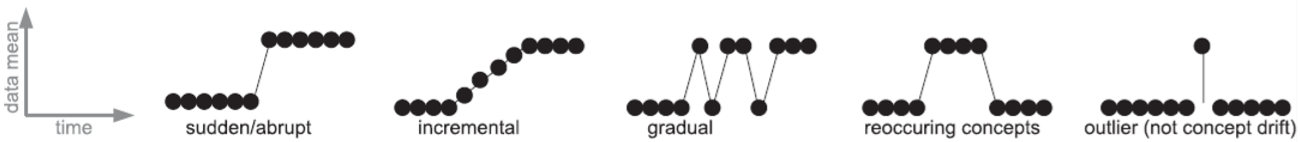
\includegraphics[width=.95\textwidth]{imgs/types_concept_drift.png}
	\caption{\label{formes_cd}Les différentes formes de Concept drift (extrait de \cite{Gama2014})}
\end{figure}

\begin{exemple}
Le changement \emph{abrupt} correspond à un utilisateur qui parle du jour au lendemain d'un nouveau sport sans jamais reparler de l'ancien.
Le changement \emph{incrémental} correspond au cas où l'utilisateur parle de plus en plus d'un nouveau sport et moins en moins de l'ancien.
Le changement \emph{graduel} représente un sport suivit la semaine et un second sport suivit uniquement lors des week-ends et/ou les vacances.
Le changement \emph{récurrent} est un utilisateur qui regarde la coupe du monde de football tout les 4 ans sans parler de football en dehors de cet évènement.
Le \emph{bruit} serait un message isolé parlant d'un autre sport.
\end{exemple}
\end{mydef}

%%%%%%%%%%%%%%%%%%%%%%%%%%%%%
%%%%%%%%%%%%%%%%%%%%%%%%%%%%%

\section{Méthodes}
\label{methodes}

Cette partie a pour but de présenter les différentes méthodes existantes pour la gestion du concept drift. Pour cela, le plan sera inspiré du classement proposé par \cite{Gama2013}. Toutes les méthodes ne seront pas présentées par manque de place, seules les méthodes applicables à notre problématique seront introduites.
%%%%%%%%%%%%%%%%%%%%%%%
%%%%%%%%%%%%%%%%%%%%%%%
\subsection{Module de mémorisation}
La mémorisation d'informations lors d'une acquisition de données par un flux est difficile car, nous ne connaissons pas la taille du flux, ni même si il se terminera (flux de tweets). Il faut donc mettre en place des stratégies de mémorisation pour ne retenir que le minimum de messages nécessaires.

\textbf{Gestion des données. } La première contrainte est de déterminer le nombre d'exemples à garder. Pour cela, les méthodes créées peuvent se classer en deux catégories :1) \emph{Exemple seul} Il est possible de ne garder qu'un seul exemple en mémoire. Cela implique d'adapter le modèle à chaque arrivée d'un exemple et de ne plus avoir accès aux exemples précédents ultérieurement. À chaque exemple $X$ reçu à l'instant $t$, on prédit une valeur $\widehat{y}_t$. Une fois la vraie valeur de la variable cible $y_t$ récupérée, on calcule la perte (voir partie \ref{estimation_de_pertes}) et on adapte le modèle. On retrouve ce principe dans l'algorithme $WINNOW$ \cite{Littlestone1988}; 2) \emph{Exemples multiples} La seconde méthode pour mémoriser les exemples est de gérer une fenêtre contenant un certain nombre d'exemples. L'algorithme $FLORA$ a été un des premiers systèmes d'apprentissage incrémental supervisé et utilise un système de mémoire à plusieurs exemples \cite{Widmer1996}. Deux approches sont possibles pour définir les exemples mémorisés : 1) Mémoriser les $n$ exemples les plus récents, ce qui permet d'utiliser les algorithmes avec le même nombre d'exemples à chaque utilisation. 2) Mémoriser les exemples récents durant une durée $t$. Cela implique de ne pas connaître le nombre d'exemples mais permet une mise à jour régulière du modèle.

\textbf{Mécanisme d'oubli} Afin d'améliorer les performances du modèle, il peut être nécessaire de supprimer certains exemples devenus obsolètes. La méthode s'appliquant \textit{a priori} le mieux à ce stage est l'oubli progressif.
Un coefficient est associé à chaque exemple, le plus souvent représentant son âge. Plus l'exemple est ancien, plus son coefficient est faible et donc l'exemple sera moins pertinent car ayant un poids plus faible. On retrouve cette approche dans \cite{koychev2000adaptation}.

%%%%%%%%%%%%%%%%%%%%%%%
%%%%%%%%%%%%%%%%%%%%%%%
\subsection{Module Détection de changement}
Cette partie présente le système qui valide ou non la présence d'un (ou plusieurs) nouveau(x) concept(s). Trois méthodes peuvent s'appliquer: 

 \textbf{Maîtrise statistique des procédés - Statistical Process Control (SPC)}
Cette technique, initialement prévue pour contrôler la qualité d'une chaîne de production, est basée sur une analyse statistique. Pour un ensemble d'exemples, l'erreur est une variable aléatoire des essais ($trials$) de Bernouilli. La distribution polynomiale donne une forme générale de la probabilité alors qu'une variable aléatoire représente le nombre d'erreurs dans l'ensemble de $n$ exemples \cite{Klinkenberg1998}. Pour chaque temps $t$ dans la séquence, le taux d'erreurs est la probabilité $q_t$ d'observer une prédiction fausse ($\widehat{y}_t \ne y_t$) et une déviation standard $\sigma_t = \sqrt{\frac{q_t(1-q_t)}{t}}$.
Le système gère deux valeurs $q_{min}$ et $\sigma_{min}$ durant l'exécution. Après avoir effectué la prédiction et avoir vérifié sa validité, on teste si $p_{t} + \sigma_{t} < q_{min} + \sigma_{min}$.
%Si cette relation est vérifiée, on affecte à $p_{min}$ et $\sigma_{min}$ respectivement les valeurs $p_{t}$ et $\sigma_{t}$.x
%
%Supposons qu'au temps ${t'}$ un exemple $(X_{t'},y_{t'})$ arrive et que le modèle de prédiction soit caractérisé par $p_{t'}$ et $\sigma_{t'}$. Le système est défini en $3$ états : \emph{In-Control} : Si $p_{t'} + \sigma_{t'} < p_{min} + 2 *\sigma_{min}$. L'exemple $X_{t'}$ est considéré comme provenant de la même distribution que les exemples précédents. \emph{Out-Control} : Si $p_{t'} + \sigma_{t'} \geq p_{min} + 3 *\sigma_{min}$. L'exemple $X_{t'}$ a une grande probabilité de provenir d'une autre distribution par rapport aux exemples précédents. \emph{Warning} : État entre les deux précédents, le taux d'erreur augmente mais n'est pas assez important pour être considéré comme "Out-Control". Cet état ne peut être final, et a besoin de plus d'exemples pour entrer dans l'un des états ci-dessus.
%%%%%%
%%%%%%

 \textbf{Gestion de deux distributions}
Ces méthodes reposent sur l'utilisation d'une fenêtre de taille fixe résumant les informations passées et d'une seconde fenêtre de taille dynamique contenant les exemples récents. La technique se base sur la comparaison statistique des distributions entre les deux fenêtres en admettant l'hypothèse nulle que les distributions sont égales.
Si celle-ci est rejetée, cela implique la présence d'un nouveau concept au début de la fenêtre dynamique  \cite{Kifer2004}.
\cite{Vorburger2006} présente une métrique basée sur l'entropie pour différencier les distributions entre les deux fenêtres. Un changement de concept est signalé lorsque la mesure passe en dessous d'un seuil fixé par l'utilisateur.

%%%%%%
%%%%%%
 \textbf{Approche contextuelle}
L'approche contextuelle se base sur l'utilisation du time-stamp de l'exemple comme étant un feature à part entière. Pour cela deux étapes sont réalisées : 1) Un arbre de décision est construit sur les exemples , si l'attribut temporel a été utilisé dans l'arbre de décision comme étant un élément discriminant entre les exemples, cela suppose plusieurs contextes; 2) Dans un second temps, l'algorithme $C4.5$ \cite{Quinlan2014} est utilisé pour déterminer les concepts intermédiaires (temporels). Cette idée est utilisé dans l'algorithme $Incremental$ $Fuzzy$ $Classification$ $System$ ($IFCS$) \cite{Bouchachia2011}.

%%%%%%%%%%%%%%%%%%%%%%%
%%%%%%%%%%%%%%%%%%%%%%%
\subsection{Module Apprentissage}

Une fois le changement de concept détecté, il est nécessaire de créer de nouvelles règles pour satisfaire les nouveaux exemples. Dans ce cas, il existe deux approches possibles : recréer le modèle ou l'adapter.
 
\textbf{Ré-apprentissage du modèle}
Dans l'hypothèse où les exemples ont été stockés en mémoire, il est possible de réapprendre le modèle à chaque nouvel exemple. Pour cela, le modèle est oublié, le nouvel exemple fusionné avec le corpus d'anciens exemples, et un nouveau modèle est appris \cite{klinkenberg2000detecting}.
Deux autres approches permettent de modifier petit à petit le même modèle.
La méthode  \emph{Incrémentale} traite les nouvelles données une à une et met à jour les données statistiques du modèle (résumé des données) à chaque fois \cite{Hulten2001}.
La méthode  \emph{Online} effectue une mise à jour du modèle avec les exemples récents. La mise à jour du modèle s'effectue en fonction des erreurs de classement \cite{Littlestone1988}.

\textbf{Méthodes adaptatives} Afin de satisfaire au maximum le modèle, il est nécessaire de générer de nouvelles règles mais il n'est pas obligatoirement nécessaire de mettre à jour toutes les règles du modèle. Certaines approches mettent en place des méthodes pour réapprendre localement.
\emph{Remplacement global} : Lors d'utilisation de méthodes adaptatives (classifieurs discriminants par exemple), on construit entièrement le modèle lorsqu'un changement de distribution est détecté \cite{Gama2004}.
\emph{Remplacement local} : Contrairement au remplacement global, si l'on détecte un changement dans une zone on remplace uniquement cette partie (sous-modèle). \cite{Carmona-Cejudo2011} utilisent cette méthode pour la classification de mails, où une catégorie de mail peut être modifiée et donc devoir être réapprise sans nécessairement nécessiter un réapprentissage de tous les autres concepts. Un changement de classification des mails de sports n'affectera pas nécessairement la classification des mails ne parlant pas de sport.

Pour gérer le modèle, deux approches sont également possibles :
 \textbf{Ensemble de modèles} La gestion de plusieurs modèles peut se catégoriser par trois approches qui ne sont cependant pas disjointes. Elles permettent, au contraire, de meilleurs résultats si plusieurs approches sont implémentées simultanément.
La \emph{gestion de modèles actifs de type "pool"} se base sur la création et la mémorisation de multiples modèles et en associe certains afin de s'adapter à la distribution actuelle \cite{Tsymbal2008}.
La \emph{sélection de modèles} qui effectue une mise à jour continue des règles d'apprentissages tels que les règles d'apprentissages sont soit recyclés dans un mode "batch" soit misent à jour 'online' en utilisant de nouvelles données \cite{Fern2003}.
Les \emph{modèles pondérés} sont valorisés selon la cohérence entre leur distribution associée et la distribution réelle. Ainsi, plus un modèle sera pertinent plus son poids sera grand. Un  modèle est actif si son poids est supérieur à un seuil fixé par l'utilisateur. Les règles d'apprentissages sont activées ou désactivées selon leur poids \cite{Kolter2003}.

 \textbf{Concepts récurrents}
Comme cité dans la définition \ref{types_concept_drift} (page \pageref{types_concept_drift}), il existe un type appelé \emph{récurrent} qui nécessite un traitement spécial car il peut avoir des conséquences sur la quantité de calcul et de traitement. Ce type définit les concepts qui disparaissent et réapparaissent régulièrement. De part les mécanismes d'oubli, les modèles associés seront oubliés et devront être réappris lors de la réapparition du concept ayant pour conséquence le calcul, une nouvelle fois, des modèles associés. De plus, lors de l'apparition d'un nouveau concept, il est nécessaire de demander à un expert de l'étiqueter. Or, cela a été fait au moment de la première apparition du concept. \cite{Masud2011} propose de garder en mémoire les anciens modèles et de ne pas les supprimer. Pour ne pas qu'ils interfèrent avec les modèles actuels, ils sont placés dans un second ensemble de modèles. Lorsqu'un changement de concept est détecté, les modèles mis de côté sont testés. Si un ancien concept est reconnu, il sera utilisé en tant que concept récurrent, sinon un nouveau concept est déclaré.

%%%%%%%%%%%%%%%%%%%%%%%
%%%%%%%%%%%%%%%%%%%%%%%
\subsection{Module Estimation des pertes}
\label{estimation_de_pertes}

Une approche très utilisée est la gestion de deux fenêtres : une première de petite taille contenant les exemples les plus récents et une plus grande contenant plus d'exemples récents (comprenant ceux de la petite fenêtre). Elles sont respectivement plus réactive et plus conservatrice. Quand un changement apparaît, il est reconnu en premier sur la fenêtre de petite taille. De façon semblable, il est possible de réaliser ce test avec des fenêtres glissantes (lorsqu'un nouvel exemple arrive, seulement le plus ancien est oublié). Basé sur cette hypothèse, \cite{Gama2013} propose d'améliorer le test $PH$\cite{Page1954} avec le ratio de deux estimations d'erreurs : une estimation d'erreur à long terme sur la grande fenêtre (ou dans le cas d'une fenêtre temporelle, un coefficient proche de 1) et un second plus petit pour la deuxième fenêtre. Un changement est signalé lorsque le ratio de ces deux estimations croît significativement.

%%%%%%%%%%%%%%%%%%%%%%%%%%%%%%%%%%%
%%%%%%%%%%%%%%%%%%%%%%%%%%%%%%%%%%%
\section{Évaluation}

\begin{mydef}[Vraie et fausse alarme]
Lorsque le module de détection de changement répond positivement, il se peut qu'il ne s'agisse pas réellement d'un concept drift mais  d'un exemple isolé. Si un nouveau concept est détecté et qu'il existe réellement, on parle de \emph{vraie alarme}, si il s'agit de bruit et que le module n'aurait pas dû répondre positivement, on parle de \emph{fausse alarme}.
\end{mydef}

\cite{Gama2013} détermine différentes métriques et une méthodologie pour désigner la pertinence d'une approche. Toutes les mesures présentées ici peuvent être calculées grâce à des données synthétiques construites de manière à connaître les changements de concepts à l'avance.
Afin de déterminer les performances de chaque approche, il est important de définir les notions sur lesquelles seront basées ces tests. Une première possibilité est d'utiliser les métriques traditionnelles que sont la \emph{précision}, le \emph{rappel} et l'\emph{accuracy}.

 \begin{multicols}{2}
\begin{tabular}{|c|c|c|c|}
	\cline{3-4}
	\multicolumn{2}{c|}{}&\multicolumn{2}{|c|}{Valeurs réelles}\\
	\cline{3-4}
	\multicolumn{2}{c|}{}&Positif&Négatif\\
	\hline
	Valeurs&Positif&VP&FP\\
	\cline{2-4}
	prédites&Négatif&FN&VN\\
	\hline
	\end{tabular}
\vfill
\columnbreak
\begin{itemize}
\item Précision : $\frac{VP}{VP+FP}$
\item Rappel : $\frac{VP}{VP+FN}$
\item Accurracy : $\frac{VP+VN}{VP+VN+FP+FN}$
\end{itemize}
\end{multicols}
 Les mentions $VP$, $FP$, $VN$ et $FN$ représentent respectivement les \emph{vrais positifs}, \emph{faux positifs}, \emph{vrais négatifs} et \emph{faux négatifs}.

 Certaines approches sont plus spécifiques aux problématiques du concept drift.
Une première catégorie de métriques liées au concept drift est celle de l'apprentissage. Il est nécessaire de savoir mesurer le coût mémoire utilisée par le processus. Pour cela \cite{Bifet2010a} propose l'unité de mesure $RAM-Hour$ qui correspond au nombre de GB de RAM utilisé par le processus en une heure.
Une métrique complémentaire est le \emph{Kappa-Statistic} qui est une mesure statistique pour déterminer la cohérence des concepts en prenant en compte le déséquilibre des  concepts. Il est calculé par $\frac{a-a_r}{1-a_r}$, où $a$ est la valeur d'accuracy d'un classifieur intelligent et $a_r$ l'accuracy d'un classifieur aléatoire qui permute les prédictions du classifieur intelligent. Le résultat de Kappa-Statistic est une valeur entre $0$ et $1$, où $0$ signifie  que la précision atteinte est aléatoire.

\paragraph{Schéma d'expériences}
Une méthode utilisée habituellement pour comparer des approches est la \emph{cross-validation}. Cependant, cette méthode n'est pas applicable ici car cela mélangerait l'ordre dans le temps des données. Une solution possible est de faire des "snapshots" à différents moments durant la création du modèle, autrement dit de récupérer à plusieurs instants toutes les données disponibles. Il est alors possible de voir les différentes étapes à la création du modèle.

Il existe deux approches possibles pour l'évaluation des techniques d'apprentissages supervisées adaptatives :1) \emph{Holdout} Lorsque la taille de l'ensemble des données étudiées est grande, la \emph{cross-validation} prend trop de temps, on mesure alors la performance sur un ensemble de données fixé. Cette méthode est surtout efficace lorsque la division entre l'apprentissage et les tests a été prédéfinie, de sorte que les résultats des différentes études puissent être directement comparés. Lors de l'essai d'un modèle à l'instant $t$, l'ensemble de maintien représente exactement le même contexte à ce moment $t$. Cependant, il n'est pas toujours possible d'utiliser cette approche car il n'est pas toujours possible de savoir avec certitude quels exemples appartiennent à un concept à l'instant $t$; 2) \emph{Prequential} Cette approche utilise les exemples courants en les appliquant au modèle avant d'adapter celui-ci. En effectuant les tests avant l'adaptation du modèle, on teste le modèle avec des situations jamais rencontrées auparavant. Ce système a l'avantage de n'utiliser aucun ensemble de maintien pour le test et utilise des données disponibles.


\subsubsection{Performance par Benchmark}
Pour effectuer une analyse comparative sur plusieurs méthodes, il faut utiliser des ensembles de données (datasets) et des implémentations logicielles des algorithmes à comparer. Il existe deux types de données: artificielles ou réelles. Dans les données artificielles, les concepts, changements de concepts sont connus. Toutefois, des données réelles sont également intéressantes car correspondant au monde réel. Il existe des données intermédiaires où les données sont initialement réelles mais certains changements de concepts sont forcés. On peut citer les jeux de données issues du framework $MOA$\footnote{http://moa.cms.waikato.ac.nz/details/} : 1) \emph{Synthétiques} : SEA Concepts Generator, STAGGER Concepts Generator, ... 2) \emph{Réels} : Text Mining, Electricity, Email Spam, Business oriented, Games.
%%%%%%%%%%%%%%%%%%%%%%%%%%%%%%
%%%%    chapitre CONCLUSION  %%%%
%%%%%%%%%%%%%%%%%%%%%%%%%%%%%%

\chapter{Conclusion} 

%Comme présenté dans cet état de l'art, le sujet du \emph{concept drift} a été le sujet de nombreux travaux et possède une multitude d'approches différentes. De plus, il s'agit d'un sujet en cours d'étude.

%L'autre sujet majeur de cette étude, l'analyse de sentiments, est aussi un sujet relativement étudié. Cependant, la combinaison des deux n'a pas souvent été une problématique abordé.

\section{Plan de stage}
Les perspectives pour ce stage sont :
\begin{itemize}
\item \emph{L'analyse de sentiments} : L'utilisation de données réelles (Données fournies par l'OADI notamment) pour apprendre des modèles est important afin d'utiliser des règles applicables aux exemples de test qui seront aussi des données réelles. Les travaux de \cite{Silva2011} se montrent très intéressants mais en posant la problématique de l'ordre des mots et la distance entre les mots recherchés, les résultats peuvent être sûrement améliorés (Une phrase ayant les deux mots clés d'une règle mais où ces mots sont espacés de plusieurs mots ne sera pas reconnue, ie. très faible probabilité qu'il soit en lien dans la phrase). Enfin, il est intéressant de réaliser une analyse de sentiments hybride sur les données en associant les deux approches ci-dessus.

\item \emph{Concept drift} : Il est nécessaire de sélectionner pour chaque module les méthodes adaptées à la problématique du stage. Ainsi, le mécanisme d'oubli devra obligatoirement être \emph{graduel} car l'âge d'un message est important (Un message posté la semaine dernière est plus important qu'un message âgé d'un an). Concernant la détection de changements, deux méthodes sont possibles : 1) La comparaison de deux distributions ; 2) Approche contextuelle (Si une personne présente une baisse de moral, il est probable que son comportement change et donc que les message soient différent après un instant précis)

Les utilisateurs ne postant pas fréquemment (en comparaison avec la vitesse de traitement d'un ordinateur), il peut être intéressant d'utiliser une méthode d'apprentissage \emph{incrémentale}. Quant à la gestion des modèles, il s'agit de combiner les approches \emph{sélectives} et \emph{pondérées} pour permettre une mise à jour facile des différents modèles.
Enfin, il est très important que l'application prenne en compte les concepts récurrents afin de détecter le plus rapidement possible un état déjà atteint par une personne.

\item \emph{Application de l'étude} : Une application de cette étude serait de détecter des personnes à risque sur des réseaux sociaux tel que Facebook ou Twitter. De plus, les résultats de la détection de changement seront intégrés comme un indicateur dans une interface développée dans l'équipe et à destination des professionnels de santé (résultat d'un TER PRO en 2015).
\end{itemize}

\bibliographystyle{plain}
% apalike pour AuteurDate
% plain pour des references numeriques

\bibliography{Stage}
\end{document}
%%% Local Variables: 
%%% mode: latex
%%% TeX-master: t
%%% End:  
 